
\documentclass[conference]{IEEEtran}

\usepackage{cite}
\usepackage{amsmath,amssymb,amsfonts}
\usepackage{algorithmic}
\usepackage{graphicx}
\usepackage{textcomp}
\usepackage{bm}
\usepackage{upgreek}

%\usepackage[retainorgcmds]{IEEEtrantools}

\usepackage[nottoc]{tocbibind}


\linespread{1.3}


\title{Predictive Distribution Estimation for Bayesian Machine Learning using a Dirichlet Prior}

%\author{Paul Rademacher}
\author{\IEEEauthorblockN{Paul Rademacher}
\IEEEauthorblockA{Naval Research Laboratory}}


%\graphicspath{ {C:/Users/Paul/Documents/PhD/Dissertation/Documentation/Figures/} }
\graphicspath{ {../Figures/} }


\DeclareMathOperator*{\argmin}{arg\,min}
\DeclareMathOperator*{\argmax}{arg\,max}

\DeclareMathOperator{\xrm}{\mathrm{x}}
\DeclareMathOperator{\Xrm}{\mathrm{X}}
\DeclareMathOperator{\yrm}{\mathrm{y}}
\DeclareMathOperator{\Yrm}{\mathrm{Y}}
\DeclareMathOperator{\Drm}{\mathrm{D}}
\DeclareMathOperator{\nrm}{\mathrm{n}}
\DeclareMathOperator{\nbarrm}{\bar{\mathrm{n}}}
\DeclareMathOperator{\zrm}{\mathrm{z}}

\DeclareMathOperator{\Prm}{\mathrm{P}}
\DeclareMathOperator{\prm}{\mathrm{p}}
\DeclareMathOperator{\Erm}{\mathrm{E}}
\DeclareMathOperator{\Crm}{\mathrm{C}}

\DeclareMathOperator{\Xcal}{\mathcal{X}}
\DeclareMathOperator{\Ycal}{\mathcal{Y}}
\DeclareMathOperator{\Dcal}{\mathcal{D}}
\DeclareMathOperator{\Ncal}{\mathcal{N}}
\DeclareMathOperator{\Zcal}{\mathcal{Z}}
\DeclareMathOperator{\Hcal}{\mathcal{H}}
\DeclareMathOperator{\Fcal}{\mathcal{F}}
\DeclareMathOperator{\Rcal}{\mathcal{R}}
\DeclareMathOperator{\Mcal}{\mathcal{M}}
\DeclareMathOperator{\Scal}{\mathcal{S}}
\DeclareMathOperator{\Pcal}{\mathcal{P}}
\DeclareMathOperator{\Lcal}{\mathcal{L}}

\DeclareMathOperator{\Rbb}{\mathbb{R}}
\DeclareMathOperator{\Nbb}{\mathbb{N}}
\DeclareMathOperator{\Zbb}{\mathbb{Z}}

\DeclareMathOperator{\Dir}{\mathrm{Dir}}
\DeclareMathOperator{\DM}{\mathrm{DM}}
\DeclareMathOperator{\Mult}{\mathrm{Mult}}
\DeclareMathOperator{\DP}{\mathrm{DP}}









\begin{document}

\maketitle

\begin{abstract}
In Bayesian treatments of machine learning, the success or failure of the estimator/classifier hinges on how well the prior distribution selected by the designer matches the actual data-generating model. This paper assumes a Dirichlet prior over a finite set and assesses the mismatch between the true predictive distribution and the distribution approximated using the training data. It is shown that highly subjective Dirichlet priors can overcome the burden of a limited training set when well matched to the true distribution, but will degrade the approximation if the prior estimate is poor. A bias/variance tradeoff will be demonstrated with illustrative examples.
\end{abstract}



\section{Extended Summary}

This article investigates how a Bayesian perspective influences the predictive distributions used to make decisions in machine learning applications. The efficacy of Bayesian learning methods depends on how well the prior knowledge imparted by the designer matches the true data-generating PMF $\uptheta$. The chosen prior distribution $\prm(\uptheta)$ over the set of data-generating probability mass functions (PMF) reflects the users confidence that different PMF's $\uptheta$ are responsible for generating the observed training data $\Drm = (\Yrm,\Xrm)$ and the novel pair $(\yrm,\xrm)$. The elements $(\yrm,\xrm)$ are characterized by $\Prm(\yrm,\xrm | \uptheta) = \uptheta(\yrm,\xrm)$ and the training data by
\begin{IEEEeqnarray}{rCl}
\Prm\big( \Drm | \uptheta \big) & = & \prod_{n=1}^N \uptheta \big(\Yrm_n,\Xrm_n \big) \\
& = & \prod_{y \in \Ycal} \prod_{x \in \Xcal} \uptheta(y,x)^{\bar{N}(y,x;\Drm)} \nonumber \;,
\end{IEEEeqnarray}
where the dependency on $\Drm$ is expressed though a transform function
\begin{IEEEeqnarray}{rCl}
\bar{N}(y,x;D) & = & \sum_{n=1}^N \delta \left[ y,Y_n \right] \delta \left[ x,X_n \right] \;.
\end{IEEEeqnarray}
The random elements $\xrm$ and $\Drm$ are observable and provide predictive information about the unobserved value $\yrm$.

If a highly subjective prior $\prm(\uptheta)$ is chosen that strongly weights the actual data PMF, low risk learning functions are possible even with limited training data $\Drm$; however, if the prior is poorly selected, a good solution will never be achieved. Conversely, a non-informative prior that treats the different PMF's will always be able to adapt will enough training data; if data is limited, however, the learning function may not deliver the required performance.

This article assumes that the prior distribution is Dirichlet. The Dirichlet PDF for the model $\uptheta \in \Theta$ is \cite{bishop}
\begin{IEEEeqnarray}{rCl}
\prm(\uptheta) & = & \beta(\alpha)^{-1} \prod_{y \in \Ycal} \prod_{x \in \Xcal} \uptheta(y,x)^{\alpha(y,x) - 1} \;,
\end{IEEEeqnarray}
where the user-selected PDF parameters $\alpha : \Ycal \times \Xcal \mapsto \Rbb^+$ are introduced and $\beta$ is the generalized beta function.

The class of Dirichlet probability density functions (PDF) have the desirable properties of full support over the set of possible PMF's and a tractable posterior distribution for independently and identically distributed data \cite{ferguson}. The full support is necessary to ensure that the true underlying model can be identified with enough training data. 

Additionally, control of the Dirichlet parameters can enable both objective and subjective prior distributions. The parameter $\alpha$ controls around which models $\uptheta$ the PDF concentrates and how strongly. For convenience, introduce the concentration parameter $\alpha_0 \equiv \sum_{y \in \Ycal} \sum_{x \in \Xcal} \alpha(y,x)$. 

Of specific interest is how $\prm(\uptheta)$ changes as the concentration parameter approaches its limiting values. For $\alpha_0 \to \infty$, the PDF concentrates at its mean, resulting in
\begin{IEEEeqnarray}{rCl}
\prm(\uptheta) & = & \delta\left( \uptheta - \frac{\alpha}{\alpha_0} \right) \;.
\end{IEEEeqnarray}
Conversely, for $\alpha_0 \to 0$, the PDF trends toward
\begin{IEEEeqnarray}{rCl}
\prm(\uptheta) & = & \sum_{y \in \Ycal} \sum_{x \in \Xcal} \frac{\alpha(y,x)}{\alpha_0} \delta\big( \uptheta - \delta[\cdot,y] \delta[\cdot,x] \big) \;,
\end{IEEEeqnarray}
which distributes its weight among the $|\Ycal| |\Xcal|$ models with an $\ell_0$ norm satisfying $\| \theta \|_0 = 1$. These trends are demonstrated in Figure \ref{fig:P_theta}. 
\begin{figure}
\centering
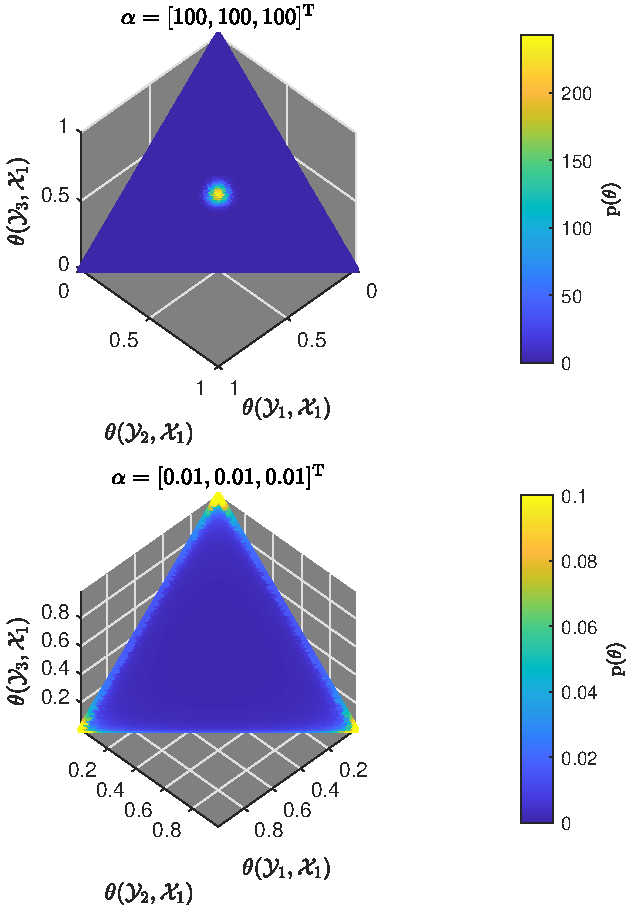
\includegraphics[width=1\linewidth]{P_theta.pdf}
\caption{Model prior PDF $\prm(\uptheta)$ for different concentrations $\alpha_0$}
\label{fig:P_theta}
\end{figure}



The metric guiding the design is the conditional expected loss, or conditional ``risk'',
\begin{equation} \label{eq:risk_cond}
\Rcal_{\Theta}(h ; \uptheta) = \Erm_{\Drm | \uptheta} \bigg[ \Erm_{\yrm,\xrm | \uptheta} \Big[ \Lcal\big( h,\yrm \big) \Big] \bigg] \;,
\end{equation}
where $\Lcal$ is the user-specified loss function. 



If the model $\uptheta$ were known, for a given set of observations a ``clairvoyant'' decision $h \in \Hcal$ could be made that is dependent only on the true predictive distribution $\Prm(\yrm | \xrm,\uptheta)$. However, as the model $\uptheta$ is not observed, the prior distribution is assumed and the Bayes risk can be formulated as
\begin{IEEEeqnarray}{rCl} \label{eq:risk}
\Rcal(h) & = & \Erm_{\uptheta}\big[ \Rcal_{\Theta}(h ; \uptheta) \big] \\
& = & \Erm_{\xrm,\Drm}\Big[ \Erm_{\yrm | \xrm,\Drm} \big[ \Lcal(h,\yrm) \big] \Big] \nonumber
\end{IEEEeqnarray}
Now, the decision is generated using the predictive distribution 
\begin{IEEEeqnarray}{rCl}
\Prm(\yrm | \xrm,\Drm) & = & \frac{\Prm(\yrm,\xrm | \Drm)}{\Prm(\xrm | \Drm)} = \frac{\alpha(\yrm,\xrm) + \bar{N}(\yrm,\xrm;\Drm)}{\alpha'(\xrm) + N'(\xrm;\Drm)} \\
& = & \left(\frac{\alpha'(\xrm)}{\alpha'(\xrm) + N'(\xrm;\Drm)}\right) \frac{\alpha(\yrm,\xrm)}{\alpha'(\xrm)} \nonumber \\
&& \quad + \left(\frac{N'(\xrm;\Drm)}{\alpha'(\xrm) + N'(\xrm;\Drm)}\right) \frac{\bar{N}(\yrm,\xrm;\Drm)}{N'(\xrm;\Drm)} \nonumber \;,
\end{IEEEeqnarray}
where $\alpha'(x) \equiv \sum_{y \in \Ycal} \alpha(y,x)$ and $N'(x;D) = \sum_{n=1}^N \delta \left[ x,X_n \right]$. This PMF can be interpreted as an estimate of the true predictive distribution $\Prm(\yrm | \xrm,\uptheta)$.



This representation of the predictive PMF views the distribution as a convex combination of two conditional distributions. The first distribution $\Prm(\yrm | \xrm) = \alpha(\yrm,\xrm) / \alpha'(\xrm)$ is independent of the training data and based on the prior knowledge implied via the model PDF parameter; the second distribution is the conditional empirical PMF and depends on $\Drm$, not on $\alpha$. For both, only those values $\alpha$ and $\Drm$ corresponding to the observed value $\xrm$ influence the distribution. 


It is informative to compare the Bayesian predictive distribution $\Prm(\yrm | \xrm,\Drm)$ to the unobserved predictive PMF $\Prm(\yrm | \xrm,\uptheta)$ and investigate the effects of subjective prior knowledge. As $\bar{N}(\Drm)$ is a sufficient statistic for the training data, any distributions dependent on $\Drm$ will be replaced by their corresponding distributions of $\nbarrm \equiv \bar{N}(\Drm)$, simplifying the analysis.

For a given $\xrm$ and corresponding number of training samples $\nrm'(\xrm) \equiv \sum_{y \in \Ycal} \nbarrm(y,\xrm)$, the expected value of the estimate condtioned on the true model $\uptheta$ is
\begin{IEEEeqnarray}{L}
\Erm_{\nbarrm | \nrm',\uptheta}\big[ \Prm_{\yrm | \xrm,\nbarrm}(y | \xrm,\nbarrm) \big] \\ 
\quad = \left(\frac{\alpha'(\xrm)}{\alpha'(\xrm) + \nrm'(\xrm)}\right) \frac{\alpha(y,\xrm)}{\alpha'(\xrm)} + \left(\frac{\nrm'(\xrm)}{\alpha'(\xrm) + \nrm'(\xrm)}\right) \frac{\uptheta(y,\xrm)}{\uptheta'(\xrm)} \nonumber \;.
\end{IEEEeqnarray}
The result is a convex combination of the conditional data-independent distribution $\alpha(\cdot,x) / \alpha'(x)$ and the true conditional distribution $\uptheta(\cdot,x) / \uptheta'(x)$. 

To aid characterization of the predictive PMF estimator, define the random process $\Delta(y;\xrm,\nbarrm) \equiv \Prm_{\yrm | \xrm,\nbarrm}(y | \xrm,\nbarrm) - \Prm_{\yrm | \xrm,\uptheta}(y | \xrm,\uptheta)$. For a given $\xrm$ and corresponding number of training samples $\nrm'(\xrm)$, the bias of the conditional PMF estimate is
\begin{IEEEeqnarray}{rCl}
\mathrm{Bias}(y;\xrm,\nrm') & = & \Erm_{\nbarrm | \nrm',\uptheta}\big[ \Delta(y;\xrm,\nbarrm) \big] \\
& = & \frac{\alpha'(\xrm)}{\alpha'(\xrm) + \nrm'(\xrm)} \left( \frac{\alpha(y,\xrm)}{\alpha'(\xrm)} - \frac{\uptheta(y,\xrm)}{\uptheta'(\xrm)} \right) \nonumber 
\end{IEEEeqnarray}
and its covariance function is 
\begin{IEEEeqnarray}{L}
\mathrm{Var}(y,y';\xrm,\nrm') = \Crm_{\nbarrm | \nrm',\uptheta} \big[\Prm_{\yrm | \xrm,\nbarrm}(\cdot | \xrm,\nbarrm) \big](y,y') \\
\quad = \frac{\nrm'(\xrm)}{\big( \alpha'(\xrm) + \nrm'(\xrm) \big)^2} \left( \frac{\uptheta(y,\xrm)}{\uptheta'(\xrm)} \delta[y,y'] - \frac{\uptheta(y,\xrm)}{\uptheta'(\xrm)} \frac{\uptheta(y',\xrm)}{\uptheta'(\xrm)} \right) \nonumber \;.
\end{IEEEeqnarray}

Combining the estimator bias and variance, the squared difference between the estimate and the true conditional model is
\begin{IEEEeqnarray}{rCl}
\mathcal{E}(y,y' ; \xrm,\nrm') & = & \Erm_{\nbarrm | \nrm',\uptheta} \Big[ \Delta(y;\xrm,\nbarrm) \Delta(y';\xrm,\nbarrm) \Big] \\
& = & \mathrm{Bias}(y;\xrm,\nrm') \mathrm{Bias}(y';\xrm,\nrm') + \mathrm{Var}(y,y';\xrm,\nrm') \nonumber \;.
\end{IEEEeqnarray}

To exemplify how the model estimate $\Prm(\yrm | \xrm,\Drm)$ approximates $\Prm(\yrm | \xrm,\uptheta)$, consider a scenario with $|\Ycal| = 10$. The data-independent PMF $\alpha / \alpha_0$ and true model $\uptheta$ are shown in Figure \ref{fig:P_yx_error_N_0} - note the significant mismatch. 

Figures \ref{fig:P_yx_error_a0_0_1} and \ref{fig:P_yx_error_a0_10} show how the expected value and variance of the estimate (represented by the blue markers and error bars, respectively) change for different values of $\nrm'(x)$ and $\alpha'(x)$ . Each individual plot heading provides the error $\sqrt{\sum_{y \in \Ycal} \mathcal{E}(y,y ; \xrm,\nrm')}$ to assess the quality of the PMF estimate. 

Observe that for $\nrm'(x) = 1$, the high variance of the $\alpha'(x) = 0.1$ estimate (favoring the empirical PMF) renders it worse than the $\alpha_0 = 10$ estimate; in fact, the variance is so high that the error exceeds that of the data-independent estimate $\alpha(\cdot,x) / \alpha'(x)$ (Figure \ref{fig:P_yx_error_N_0}). Conversely, for $\nrm'(x) = 10$, the confidence of the $\alpha'(x) = 10$ estimate leads to high bias and the $\alpha'(x) = 0.1$ estimate is superior. For $\nrm'(x) = 100$, both the $\alpha'(x) = 0.1$ and $\alpha'(x) = 10$ estimates begin converging to the true predictive distribution - this is guaranteed due to the full support of the Dirichlet prior.


\begin{figure}
\centering
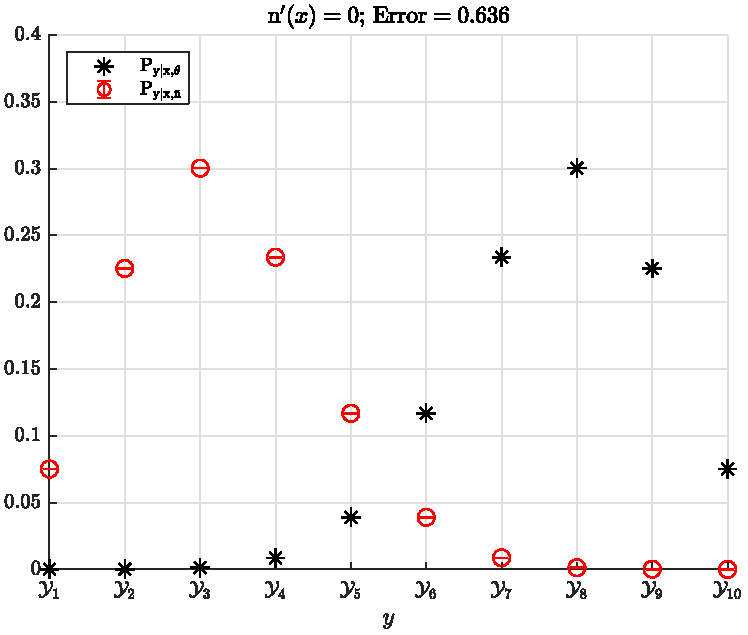
\includegraphics[width=1\linewidth]{P_yx_error_N_0.pdf}
\caption{Model $\uptheta$ estimate, no training data}
\label{fig:P_yx_error_N_0}
\end{figure}

\begin{figure}
\centering
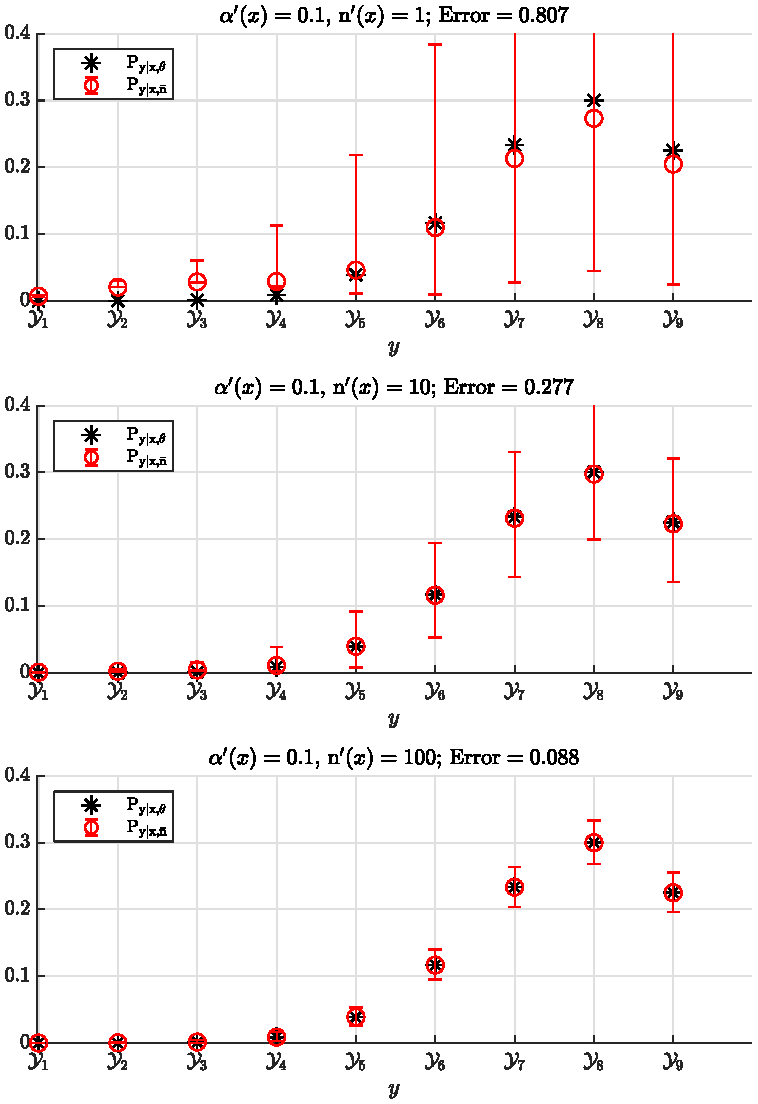
\includegraphics[width=1\linewidth]{P_yx_error_a0_0_1.pdf}
\caption{Model $\uptheta$ estimates, $\alpha_0 = 0.1$}
\label{fig:P_yx_error_a0_0_1}
\end{figure}

\begin{figure}
\centering
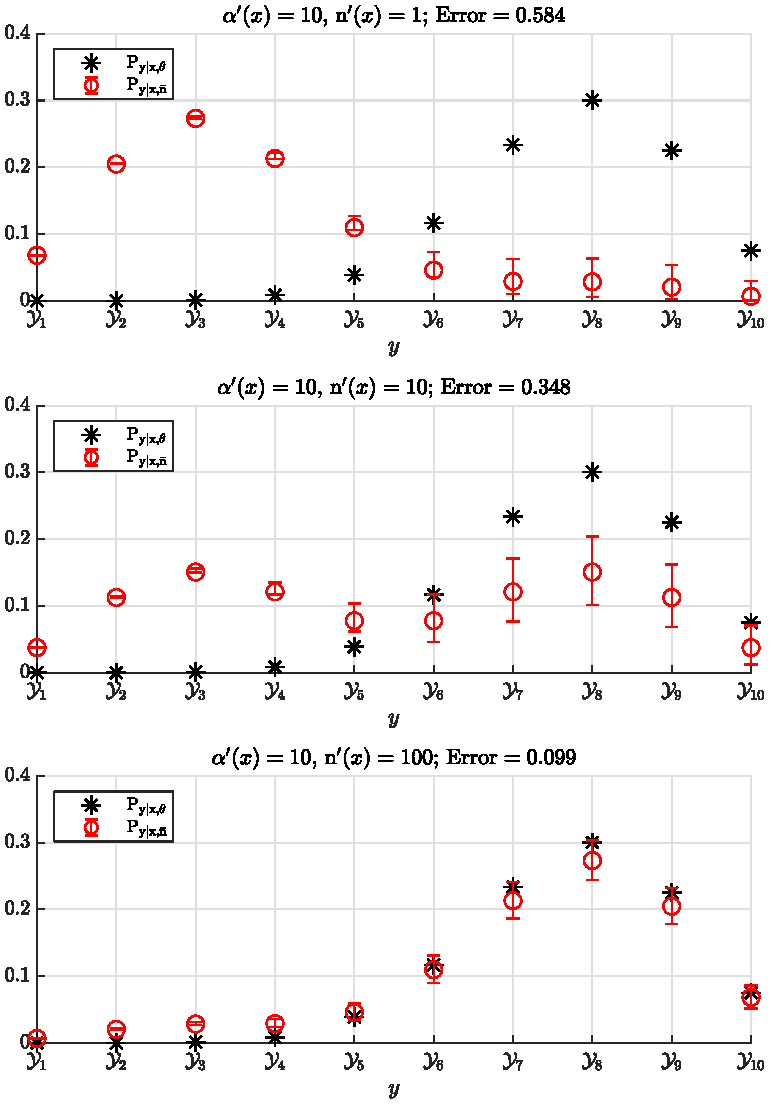
\includegraphics[width=1\linewidth]{P_yx_error_a0_10.pdf}
\caption{Model $\uptheta$ estimates, $\alpha_0 = 10$}
\label{fig:P_yx_error_a0_10}
\end{figure}


The conditional second moments of the difference between the two predicitve PMF's have important applications for Bayesian regression, specifically for determining the expected squared-error loss. This will be a primary focus of future work.






\bibliographystyle{plain}
\bibliography{{../References/phd_bib}}

\end{document}


























